% !TeX root = ../document_maitre.tex

\label{réalitéIndexationAuto}

Ce processus est né de plusieurs constats sur l'indexation des textes, notamment, dans les bases de données patrimoniales. D'abord, l'indexation des textes et objets patrimoniaux par mots-clés, comme pratiquée encore aujourd'hui, permet d'optimiser l'interrogation des bases de données. Cependant, sur de grandes quantités de données procéder à une indexation manuelle, souvent effectuée par plusieurs personnes, amène à créer de la variation là où les bases ont besoins de constances. Ajoutons que plus la cohérence et la stabilité sont basses, plus les résultats sont imprécis.\footcite[p.1]{keversIndexationSemiautomatiqueTextes2009} 

Le second constat vient de la masse documentaire à traiter et de sa typologie. Les textes concernées concerne de vaste périodes chronologiques demandant la compréhension d'un vocabulaire vaste et évolutif et donc l'adaptation des mots clés. De plus, ces collections sont en expansion constante et toujours plus rapide, ce qui demande une augmentation du rythme d'indexation. \footcite[p.1]{keversIndexationSemiautomatiqueTextes2009}

Ces deux éléments mènent à penser que l'indexation par seul moyens humains devient une limite importante des bases de données patrimoniales qui, finalement, complexifie la tâches des \gls{SRI}\newline

Mais alors pourquoi une indexation \guillemet{semi-automatisée} et pas une totalement automatisée ? Si l'automatisation totale permet d'accélérer le traitement, on remarque des défaillances importantes. Ces processus ont tendances à produire les mêmes erreurs d'indexation que les humains tout en étant moins précis dans le choix des mots utilisés.\footcite[p.1]{keversIndexationSemiautomatiqueTextes2009}

Une indexation semi-automatisée permet de faire de l'\gls{IA} un outil d'appui, capable de suggérer des indexations et de proposer une base de travail propre très rapidement\footcite[p.69 à 71]{hussonIndexationIconographiqueIntelligence2025}. L'humain n'a plus à analyser chaque document lui même: il n'est plus que le vérificateur qui peut valider la proposition issus du processus ou alors créer une alternative. En associant la vérification humaine à la rapidité de traitement de l'\gls{IA}, on vise à augmenter la pertinence et la rapidité du processus. C'est ce que l'on l'appelle l'approche \textit{Humain in the loop} : l'\gls{IA} analyse et suggère, puis l’opérateur valide, invalide ou modifie.\newline

Avant d'examiner ce qui ce fait ou non dans le cadre de l'\gls{imgani}, commençons par l'analyse du principe appliqué à des collections de musées plus statiques. Pour cela, je m'appuierai principalement sur le projet mené par Pierre Husson\footcite{hussonIndexationIconographiqueIntelligence2025}, promotion TNAH 2025, au sein du projet \textit{IconographIA} consistant en l'application de tels processus sur des tableaux italiens du RETIF\footnote{Répertoire des tableaux italiens dans les collections publiques françaises}. 

Pierre Husson met tout d'abord en avant la complexité de notion de vocabulaire \footcite[p.9 à 17]{hussonIndexationIconographiqueIntelligence2025} qui est pluriel. D'abord car adapté à chaque typologie patrimoniale et ensuite car au sein même de ces typologies existent des subdivisions avec leurs propres besoins terminologiques. Ces vocabulaires sont standardisés et contrôlés dans des \gls{thesaurus} auxquels se rattacher comme ceux du Getty Research Institute. 

Bien qu'on puisse s'appuyer sur ces outils pour contrôler la génération d'un outil d'indexation automatique\footcite[p.38 à 40]{hussonIndexationIconographiqueIntelligence2025}, il existe un fossé entre la compréhension de ce que l'\gls{IA} voit et la sémantique des thésaurus. Pierre Husson met en avant que les modèles n'ont pas eu de difficultés des formes génériques \textit{(humains, animaux, épées, etc)}. Mais reconnaître que ces formes sont des concepts artistiques, comme des représentations codifiées consignées dans les \gls{thesaurus}, est encore hors de portée.\footcite{hussonIndexationIconographiqueIntelligence2025} Ils sont de plus imprécis face aux spécificités de l'art, notamment sur la question du genre iconographiques encore complexe à déterminée malgré de récent progrès.\footcite[p.41 à 43]{hussonIndexationIconographiqueIntelligence2025}

À la lumière de ces éléments, Pierre Husson conclut que l'indexation iconographique est loin d'être un processus automatisable. Cependant, les récentes avancées notamment avec les \gls{mmlts} capables de traiter texte, images, vidéos et/ou sons en même temps, permettent d'envisager de s'appuyer dessus dans des processus semi-automatisés. \newline

Mais alors, pourquoi faire de l'indexation semi-automatisée sur l'\gls{imgani} ? La raison principale est l'explosion quantitative des collection. La Cinémathèque française conserve à titre d'exemple plus de 40 000 \oe{uvres} cinématographique.\footnote{Pour plus d'information, consulter : \url{https://www.cinematheque.fr/les-collections-de-films.html}} Cela s'explique par l'intensification de la production de film professionnel : plus de 9511 films sont réalisés à l'échelle mondiale en 2023 contre 7620 en 2016 selon le WIPO\footnote{Pour plus d'informations, consulter : \url{https://www.wipo.int/fr/web/global-innovation-index/w/blogs/2025/global-film-production}}. Cela ne prend pas en compte la production de films amateurs, et toutes \glspl{imgani} produites en dehors du cinéma. De même, cela ne prend pas en compte ce qui est déjà produit et qui continu d'être conservée ce qui créer donc un véritable phénomène de masse demandant à accélérer le processus d'indexation.

Ajoutons à cela que, tout comme les tableaux, l'\gls{imgani} pose ses propres difficultés à commencer par la notion de mouvement. Pour créer cette impression de mouvement, une \oe{uvre} d'\gls{imgani} est composée de plusieurs centaines, ou milliers, d'images capturées à la chaîne pendant un instant déterminé. Ces images sont donc porteuse de sens, surtout au sein d'ensembles que sont les \glspl{sq} et les \glspl{sc}. L'indexation de vidéos ou de films entier repose donc principalement sur l'analyse de ces images au sein de ces deux ensembles qui déterminent un sens précis. 

De plus, bien que, comme pour les tableaux, on cherche à reconnaître les entités, les personnes, les objets, et tout autre éléments, mais dans cette notion d'ensemble, l'\gls{imgani} possède ses propres besoins d'indexation. En voici les trois principaux :

D'abord, celui d'une extraction automatique des \gls{sq} ou les \gls{sc} au sein d'une \oe{uvre}, Ou bien d'\oe{uvres} au sein d'un même support, afin de proposer une indexation optimale pour des résultats de recherches précis. Disposer d'un outil capable de découper automatiquement les \oe{uvres} d'\gls{imgani} en des unités documentaires plus petites et indexées à cette échelle est essentiel.

Un second besoin est de pouvoir faire des liens entre différentes \gls{sc} et/ou \gls{sq} d'une même \oe{uvre}, ou idéalement entre différentes \oe{uvres}. Cela peut permettre de reconstituer des arcs narratifs multiples ou encore de suivre l'évolution d'un sujet d'un bout à l'autre de l'\oe{uvre}. L'idée étant de pouvoir saisir la richesse des liens caractérisant les \oe{uvres} d'\gls{imgani}. Ils peuvent être faits entre les \oe{uvres}, au sein de suites thématiques comme les duologies la notion de saisons au sein d'une série. Saisir ces liens et porosités est aujourd'hui un objectif pour certaines institutions.

Enfin l'association entre le visuel et le son, une caractéristique principale des \glspl{imgani} aujourd'hui. L'idée est d'exploiter l'\oe{uvre} et les thèmes contenus à la fois visuellement et auditivement. Par exemple une \gls{sq} triste peut être identifiée par les changements colorimétriques et émotions des acteurs, mais aussi par l'environnement sonore et les dialogues. Cela sous-entends que le processus gagnerait à pouvoir \guillemet{comprendre} le son au sein de \glspl{sc} et \glspl{sq} afin de mieux exploiter les thèmes présents.

L'ensemble de ces éléments distingue clairement le traitement d'\glspl{imgani} de celui de tableaux. Bien que les éléments à extraire peuvent être les mêmes, les spécificités de l'\gls{imgani} en complexifient fortement la détection et l'analyse. Ce qui demande donc à penser à de nouveaux outils et processus de traitement.\newline

On peut dés lors distinguer deux phases essentielles de traitement pour l'\gls{imgani}. Une phase de \guillemet{pré-traitement} pour décomposer l'\oe{uvre} ou la bande vidéo analysée en autant d'entités que nécessaire que cela soit à l'échelle des \oe{oeuvres}, \glspl{sc} ou \glspl{sq}. Et une seconde phase de traitement pour reconnaître et identifier les éléments d'indexations par l'usage de termes conforme à au moins un Thésaurus. 

Après des recherches sur le sujet, un premier constat s'offre à nous. Il n'existe pas encore de solutions \gls{ops} permettant d'effectuer cette chaîne de traitement. Des outils existent afin de réaliser certaines tâches comprises dans le processus, comme la \gls{do}, mais ils n'ont encore jamais été rassemblés. Et du côté des solutions privées, certaines solutions à destinations du monde patrimonial existent et sont déjà utilisé. Cependant elles manquent de transparence ce qui fait que nous n'avons pas connaissance de la méthodologie appliqués, des outils utilisés et des compatibilités avec des standards de descriptions.

On peut citer Archipanion que les Archives fédérales Suisses utilisent à des fins de reconnaissance et d'extraction de métadonnées sur des images et vidéos. Cette institutions a indexée plus de 200h de vidéos de l'émission \textit{Ciné-Journal} Suisse.\footcite{ArchipanionPourCineJournal} L'article reste succint et nous n'avons pour information que l'extrait suivant : \guillemet{Grâce à sa fonction de recherche par contenu visuel, Archipanion permet, en les décrivant, de rechercher des scènes ou des textes figurant dans le fonds du Ciné-Journal suisse et de trouver ainsi des contenus de manière exploratoire [...] Outre la recherche textuelle par description, Archipanion permet aussi de trouver des contenus visuels similaires au sein de la collection.}. 

Sur le site d'Archipanion\footnote{Pour plus d'information, consulter : \url{https://www.archipanion.com/fr/}} voilà les conclusions que nous pouvons établir. Le processus établit agit sur chaque images à analyser individuellement, y compris au sien d'\gls{imgani}. En s'appuyant sur de la \gls{CV} ou bien des \gls{mmlts}, il semble y avoir un processus de \gls{Vecsion} : chaque image se voit attribuer une \gls{vcs} en fonction des entités, des lieux et du style général reconnus. Lorsqu'un utilisateur interroge ces documents, l'utilisateur décrit ce qu'il souhaite trouver, donc une scène ou une image, qui est transmise à l'\gls{IA}. Cette requête est transformée en \gls{vcs} qui sont comparés à ceux des \glspl{imgani} stockées. Plus des \gls{vcs} sont proches, plus il est probable qu'il existe une correspondance. 

Des questions subsistent. Les personnes sont-elles reconnues ? Qu'en est-il des réalisateurs et équipes techniques ? Qu'elle est la précision des métadonnées générées ? Il y'a-t-il une indexation de toute l'entière de l'\oe{uvre} d'\gls{imgani} ou juste chaque image ? 



							% A REPRENDRE ICI 



L'opacité des solutions privées ne nous permet pas d'apporter des réponses à ces questions. Et les articles d'institutions utilisant cette solution ne sont pas nombreux, en réalité seul celui-ci semble exister ce qui peut s'expliquer par le caractèr récent de tels outils. Nous pouvons cependant déterminés deux choses : dans les deux sources, il n'y aucune mention de reconnaissance précises d'entités nommées. Une actrice célèbre, un monument ou encore un objet unique et identifiable ne semble être identifier suffisament précisément afin de l'indexer de cette manière. Les analyses semblent rester très générales : une voiture, une femme, un homme, etc. Ensuite, il n'y aucune mention de reconnaissance de l'architecture documentaire. Par exemple, une bobine comportant 3 \gls{oe} différentes semble être analysées comme une seule et même \gls{oe} ce qui ne permet de corriger un problème de mélange des supports et des \gls{oe} rencontrées par les institutions sur cette typologie. 

Finalement, c'est une solution assez générale appliquant des principes déjà éprouvées sur les images fixes à des objets en mouvements. L'\gls{imgani} semble être confondu avec une image statique, et est donc analysée de la même manière ce qui amène à perdre la richesse amenée par cette typologie documentaire. De plus, traiter chaque \gls{imgani} composant une \oe{uvre} représente un processus long et coûteux qui, appliqué à des collections comme celles de la Cinémathèque française, peut ne pas présenter un rapport coûts / bénéfices suffisant. \newline

Du côté des solutions dites \textit{open source}, le seul processus de traitement des \gls{imgani} connu est \textit{vitrivr-engine}\footnote{Pour plus d'informations, consulter le github du projet : \url{https://github.com/vitrivr}} développé par l'Université de Bâle, en Suisse, et sur lequel est basé la solution Archipanion. 

Cette solution est basée sur la recherche de contenu, c'est à dire qu'on offre la capacité à l'utilisateur de décrire ce qu'il recherche et de l'orienter vers le bon passage d'une vidéo.\footcite{rossettoVitrivrFlexibleRetrieval2016} 

Son architecture est modulaire, c'est à dire qu'elle se compose, ici, de 3 briques logicielles qui intéragissent ensemble mais qui ne composent pas un outil unique. Une interface d'interrogation, \textit{vitrivr-ng}, une base de donnée, \textit{Cottontail DB}, et un logiciel multimodal pour la recherche dans des documents multimédia, \textit{Cineast}. Voici un schéma du fonctionnement global applicatif : 

\begin{figure}[H]
	\centering
	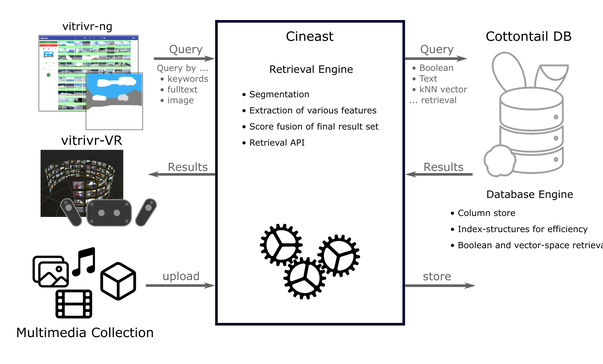
\includegraphics[width=1\textwidth]{./Schema/vitrivr.png}
	\caption{Schéma de fonctionnement de la solution vitrivr. Source : site officiel vitrivr à l'URL \url{https://vitrivr.org/vitrivr.html}.}
	\label{fig:vitrivr_fonction}
\end{figure}

Le logiciel fonctionne sur deux étapes. La première étape est celles de prétraitement des données : à l'intégration des documents multimédias dans la base de données, cela passe par \textit{Cineast} qui analyse l'\gls{imgani}, en extrait les entités visibles et lui donne un \gls{vcs} associé. La base de donnée stocke à la fois les \oe{uvres} multimédias et leurs représentations vectorielles au sein d'une base PostGreSQL adapté au stockage vectoriel \footcite{rossettoVitrivrFlexibleRetrieval2016}. La seconde étape est celle de l'interrogation utilisateurs : la requête peut être formulée de différentes manière, par phrase, par recherche de similarité avec une image ou un schémas\footcite{rossettoVitrivrFlexibleRetrieval2016}, et est d'abord vectorisée par \textit{Cineast} avant d'être envoyée à la base de données par une API. Les \gls{vcs} sont ensuite comparés, et les résultats sont renvoyés à l'utilisateur soit directement dans l'interface \textit{vitrivr-ng} soit en format 3D via \textit{vitrivr-VR}.  

Ce qui est intéressant, c'est l'absence des différentes modalités d'interrogations des documents multimédias dans la solution de Archipanion. En effet, seule la recherche par requête textuelle ou par mots-clés semble intégrée. Destinée à la gestion des collections, on peut penser que l'approche par schéma et images similaires ait été jugée non ou peu pertinente notamment dans des questions d'usages et de pratiques. 

Finalement, nous nous retrouvons un peu face aux mêmes limites pour une intégration dans le monde patrimonial. Ce logiciel est concentré sur le contenu, le visuel, mais délaisse l'aspect documentaire. Les \gls{imgani} sont annotées, identifiées, mais elles ne sont pas indexées, mises en relations, décortiquée et encore moins manipuler comme un objet patrimonial. Une institution patrimoniale avec des besoins fort en matière de gestion risque de se trouver limitée : pas d'identification des personnes, pas d'identification technique, pas de rédaction d'une notice, pas de séparation en \glspl{sc} ou \glspl{sq} ou même entre \oe{uvres}.

Nous pouvons donc conclure que les solutions proposées pour la gestion de l'\gls{imgani} par \gls{IA} sont orientées gestion des contenus et non gestion documentaires. C'est insuffisant lorsque l'on souhaite gérer une collection patrimoniale. \newline

Cela nous amène donc à voir plus large que des solutions sur étagères afin de trouver des outils permettant de répondre à l'ensemble des besoins institutionnels. Nous allons donc présenter des outils \textit{open-source} qui, articulé ensemble, peuvent amener à penser et créer une solution d'indexation complète de l'\gls{imgani}. 

\subsection{Manipulation de l'image et des \glspl{pl}}

Le premier élément est le besoin de manipulations des documents multimédias en tant que tel. Une institution patrimoniale peut souhaiter séparer différentes \oe{uvres} d'\gls{imgani} présentes sur un même support physique, ou bien une même \oe{uvres} en différentes sous-unités que sont la \gls{sc} et la \gls{sq}. Cela demande nécessairement de pouvoir manipuler le document multimédia afin de le découper à des endroits précis et de pouvoir placer des repères temporels sur ces découpages. De cette manière, on pourrait segmenter une bande vidéo en différent segments indépendant avec chacun un \guillemet{horodatage}, c'est à dire un marqueur temporel au début et à la fin du segment afin de le situer à l'échelle de l'\oe{uvre} originale. 

\label{FFmpeg}Pour cela, il existe le logiciel FFmpeg qui permet de manipuler des bandes vidéos et des bandes sons. Logiciel \textit{open-source} pouvant traiter tous les formats vidéos et audios, il est très utilisé par des plateformes multimédia comme Youtube afin de permettre de manipuler les vidéos \textit{(diffusion, manipulation du flux, etc)}. Le gros avantage de ce logiciel est sa compatibilité avec des langages de programmation comme python, qui permettent de l'intégrer dans des workflows automatisés de traitement de données assez facilement.\footnote{Pour plus d'informations, consulter : \url{https://www.ffmpeg.org/documentation.html}}\newline

Avec FFmpeg, la \gls{seg} audio et vidéos est rendue possible. Autrement dit, on peut créer un extrait d' une \oe{uvre} avec la granularité désirée. Cependant, FFmpeg demande une action humaine : il n'intègre pas de système afin de repérer des variations justifiant un découpage. \label{PyScene}L'outil PySceneDetect permet d'identifier dans une piste vidéos chaque changement de \glspl{pl}. Il fonctionne selon le principe de \textit{threshold} c'est à dire que l'utilisateur définit un palier indiquant au logiciel que toute comparaison entre image produisant un score inférieur à ce palier signifie que c'est un seul \gls{pl}. Si le score de comparaison y est supérieur, alors ce sont des \glspl{pl} différents. \footnote{Pour plus d'informations, consulter : \url{https://www.scenedetect.com/}} 

Cet outil est très intéressant : d'abord c'est une librairie python ce qui le rend parfaitement intégrable à un script automatique. On peut ainsi lier FFmpeg à PySceneDetect afin de lier la détection à l'extraction. De plus, il s'appuis sur d'autres librairie python reconnues et approuvées pour l'analyse d'image. On peut notamment penser à OpenCV, MoviePY et PyAV pour l'analyse images par images dans une vidéo ou bien d'images fixes. Ce sont des solutions très souples permettant de choisir un détecteur, c'est à dire un algorithme qui permet d'analyser une image et de la comparer avec l'image suivante afin de déterminer si il y a un changement de \gls{pl} ou non. Chaque détecteur est spécialisé sur l'analyse d'un composant de l'image, par exemple : \footnote{Pour consulter la documentation relative à chaque détecteur, consulter : \url{https://www.scenedetect.com/docs/latest/api/detectors.html}} \label{detecteurs}

\begin{enumerate}
	\item \textit{ContentDetector} : ce détecteur est le plus utilisé car le plus complet et souple. Chaque image est analysées dans son contenu notamment colorimétrique et structurel et obtient un score de détection. En fonction de cette analyse, il calcule un score pour chaque image, disons une forme de \gls{vcs}, et compare les score entre eux. La différence entre les scores est ensuite reportée au \textit{threshold}.
	\item \textit{AdaptiveDetector} : ce détecteur reprend le principe précédent. Il analyse les mêmes points, de la même manière. Le changement opère au niveau du système de comparaison. En effet, au lieu de se référer au \textit{threshold} ce détecteur calcule lui même une moyenne glissante entre les images. C'est à dire que le \textit{threshold} change automatiquement en fonction du cas présent. Cela rend le détecteur moins sensible aux mouvement de caméras, qui n'indique pas un changement de plan nécessairement. 
	\item \textit{TresholdDetector} : si les deux détecteurs précédents sont basé sur des analyses structurelles afin de repérer des coupures, celui ci s'attarde sur les pixels afin de repérer les changements plus fins comme des transitions. 
	\item \textit{HistogramDetector} : à l'échelle d'une vidéo, l'\gls{hist} est un graphique permettant de visualiser, et parfois gérer, l'équilibre entre ombres et lumières. Ce détecteur analyse cet histogramme, et compares les histogrammes des images afin de détecter des changements d'équilibre. Efficace afin d'identifier les coupures rapides. 
	\item \textit{HashDetector }: il est similaire à \textit{ContentDetector} et \textit{AdaptativeDetector} si ce n'est qu'il se base sur la création d'un \textit{hash}, c'est à dire une empreinte de taille fixe et propre à chaque image, pour chaque image. Ensuite, les \textit{hash} sont comparés et leurs écarts calculés puis mis en relation avec le \textit{threshold}\newline
\end{enumerate}

Ces détecteurs peuvent s'accumuler, permettant ainsi des analyses multiples mais alourdissant fortement le processus. Plus il y a de détecteurs, plus le traitement s'alourdis et plus on multiplie la finesse de l'analyse ce qui peut amener à faire de chaque petites variations une raison suffisante pour segmenter. 

L'extraction se fait à l'échelle du plan puisque cet outil repère les ruptures de prises de vues ce qui caractérise les différents \glspl{pl}. Les \glspl{sc} et \glspl{sq}, beaucoup plus intéressantes pour une institutions patrimoniales, ne sont pas encore saisisables par des solutions informatiques. Il est cependant tout à fait possible d'utiliser cet outil pour découper une \oe{uvre} en autant de \glspl{sc} et \glspl{sq} qui la compose. Commençons d'abord par définir ce qu'est \gls{sc} puis une \gls{sq}

Une \gls{sc} représente l'unité de base d'une \oe{uvre} d'\gls{imgani}. Il s'agit d'un ensemble de plans mettant en scènes les mêmes acteurs, dans les même lieux, souvent autour des mêmes objets et toujours autours des mêmes actions, sujets et objectifs. Ainsi, pour recréer une \gls{sc} il faut pouvoir identifier ces éléments de continuité au sein de \glspl{pl} adjacent et cela jusqu'à l'identification d'une rupture nette. Si nous sommes capables d'identifier ces éléments, on peut tout à fait penser à créer des \gls{vcs} pour chaque plan basé sur l'identification de ces éléments. Comme dans un système de \guillemet{recherche augmentée}, c'est la comparaison entre les \gls{vcs} qui va déterminer l'action et le résultat à retourner. Si au sein de \gls{pl} adjacents les \gls{vcs} sont extrêmement proche alors ils peuvent regroupé en une \gls{sc} et cela jusqu'à détecter une rupture avec un autre \gls{pl}.

Une \gls{sq} est un ensemble de \glspl{sc} regroupées autour d'éléments bien plus abstrait. Ces \glspl{sc} partagent une thématique commune, un sujet qui bien souvent sert au développement d'une partie de l'intrigue de l'\gls{oe}. En arrivant à saisir un motif, sujet ou thème commun il serait possible d'agir de la même manière que précédemment : vectoriser les \glspl{sc} sur ces éléments et rassembler les \gls{vcs} proches en \glspl{sq}. \newline

Ainsi on comprends que pour indexer une \oe{uvre} d'\gls{imgani} il faut aller bien plus loin dans le processus de traitement que la simple détection de plan autrement dit de rupture visuelle. Il faut pouvoir identifier des acteurs, et leurs apparitions dans les plans successif. Mais aussi reconnaître ou du moins caractériser en partie les lieux, parfois fictif, qui permettent d'ancrer l'action dans un élément \guillemet{concret}. En allant plus loin, il faut également des outils capable de déterminer la thématique générale des \glspl{pl} : dramatique, comique, action, etc. Ce n'est qu'a l'aide de ces éléments on peut envisager deux choses : indexer des éléments d'une \oe{uvre} et utiliser ces éléments pour créer des regroupements de \glspl{pl}.

Nous allons donc présenter des outils intégrable dans un script d'automatisation de l'indexation d'\glspl{imgani} permettant la détection et l'analyse des éléments identifiés. Comme nous l'avons déjà abordé, nous ferons l'impasse sur \newline le module \textit{Cineast} de \textit{Vitrivr}. Gardons simplement à l'esprit que ce module ne propose pas une indexation assez fine et précise et que de plus, l'\gls{imgani} est traitée comme une image fixe. Débutons par l'outil \textit{SAM 2}\footcite{SAM2Segment} et son \textit{framework} dérivé \textit{Seg2Track-SAM2}\footcite{mendoncaSeg2TrackSAM2SAM2basedMultiobject2025a}.

\subsection{\Gls{seg} d'une \gls{imgani}}

\label{SAM2} Développé par l'entreprise Meta, \textit{SAM 2} est un modèle d'\gls{IA} spécialisé en \gls{CV} afin de segmenter une image ou une vidéo : c'est à dire de détecter et isoler tout élément composant une image. Ce modèle est particulièrement intéressant pour trois spécificités : 

D'abord sa capacité de \textit{zero-shot}, c'est à dire sans être entraîné à détecter un objet spécifique, il pourra tout de même le segmenter au sein d'une image. \footcite[p.8 à 10]{raviSAM2SEGMENT2025}

Ensuite, sa capacité à recevoir des \textit{prompts} de la part de l'utilisateur, ce qui permet deux choses : de mieux diriger la \gls{seg} et de la réitérer si nécessaire dans un but d'affinage. \footcite[p.3 à 4]{raviSAM2SEGMENT2025}

Enfin, son système de mémorisation des formes détectées. Dans une \oe{uvre} d'\gls{imgani} il n'est pas rare qu'un objet soit totalement visible puis ensuite peu à peu caché par un autre élément. Ce modèle mémorise ce qu'il détecte, de cette manière si l'objet détecté est partiellement couvert à un moment donné, le modèle garde la forme initiale de l'objet. C'est particulièrement utile afin de traquer les objets. \footcites[p.4 à 5]{raviSAM2SEGMENT2025}{SAM2Segment}

Cependant, cet outil possède trois limites importantes. La première est l'absence d'une attribution et d'une gestion d'identité à des objets. Un objet détecté est gardé en mémoire, ainsi si il disparaît partiellement de l'image le modèle garde en mémoire son emplacement et sa forme. Cependant, comme il n'est pas identifié si cet objet disparaît puis réapparaît, \textit{SAM 2} le reconnaît comme un nouvel objet ce qui est faux. Appliquée à des institutions patrimoniales, l'absence de cette identification risque de poser deux problèmes : d'abord car le modèle risque de détecter constamment le même objet, et ensuite car cela complexifie la reconnaissance d'un même objet dans différentes \glspl{sq} ou \glspl{sc}. La seconde est la mise en mémoire en elle même car sur une volumétrie importante, le nombre d'objets à détecter est exponentiel ce qui alourdit la mémoire du modèle et en ralentit le traitement.\footcite[p.22 à 40]{raviSAM2SEGMENT2025} La dernière limite est l'absence de classification des objets. En effet, \textit{SAM 2} reconnaît des formes mais ne pourra pas déterminer que ceci est une voiture et ceci un vase. C'est ce que l'on appelle un modèle \guillemet{classe-agnostic} \newline

\textit{Seg2Track-SAM2} permet d'apporter quelques solutions. Cet outil est un framework permettant d'associer \textit{SAM 2} à un modèle de reconnaissance d'objet pré-entraîné comme YOLO ou bien Faster R-CNN et au module \textit{Seg2Track} qui s'occupe de gérer l'attribution et la mise en mémoire d'identifiant des objets.\footcite{mendoncaSeg2TrackSAM2SAM2basedMultiobject2025a}

L'association à un modèle de reconnaissance d'objet externe, choisi par l'institution, permet de spécialiser le \textit{framework} pour la détection de certains objets et en déterminer la nature. Ainsi on brise la nature \guillemet{classe-agnostic} de \textit{SAM 2} en apportant, par une ressource extérieure, la possibilité d'identifier des classes d'objets comme des voitures, des vases, etc. Au-delà, cela permet d'accélérer le traitement et de le fiabiliser par l'application de deux modèles. \textit{SAM 2} est surtout utilisé afin d'assurer le suivi de l'objet au travers des différents \glspl{pl} se succédant. Le module \textit{Seg2Track} permet de résoudre l'attribution d'identifiant à chaque objet identifié. En effet, ce module permet d'attribuer un identifiant à chaque objet identifié, de le garder en mémoire et de l'associer à la forme de l'objet détecté elle aussi mémorisée, et ainsi de pouvoir reconnaître si le \guillemet{nouvel objet} détecté est bien un nouvel objet ou un même objet. 

Ce \textit{framework} se place aujourd'hui comme une référence dans la segmentation d'images et d'\glspl{imgani}. Sur le jeu de données KITTI MOTS du \textit{benchmarks} KITTI, ce \textit{framework} s'est placé 4ème en 2025 sur l'analyse de ce dernier, essentiellement composé de voitures et de piétons, sans entraînement préalable. \footcite[p.5]{mendoncaSeg2TrackSAM2SAM2basedMultiobject2025a} Dans un tout autre domaine, celui de la chirurgie, ce \textit{framework} a montré des résultats prometteurs sur la \gls{seg} multi-objets en \textit{zero shot} avec notamment une possibilité de \gls{ft} en temps réel permettant de réellement fiabiliser les résultats. \footnote{Pour plus d'informations sur le sujet, voir : \footcite{yuanSystematicEvaluationGuidelines2026}} \newline

Dans l'indexation d'une \gls{imgani}, disposer d'un tel outil est pertinent. Parfois chargée en informations visuelle, l'application de \textit{SAM 2} ou du \textit{framework} \textit{Seg2Track-SAM2} permettrait de faire un tri informationnelle via une \gls{seg} de l'image. Chaque objets et personnes pouvant être détectés et isolés les uns des autres tout en étant suivis au fur et à mesure des images composant l'\oe{uvre} analysée. \newline

\subsection{La compréhension des sous-titres}

Un autre élément pouvant être analysé pour indexation ce sont les sous-titres. Ils peuvent servir d'appui afin d'extraire du sens au sein d'une \gls{sc} ou \gls{sq}. Des outils comme VideOCR\footnote{Pour plus d'informations, consulter : \url{https://github.com/timminator/VideOCR}} sont spécialisés sur le sujet et permettent d'isoler les sous-titres de l'image, et de les transcrire en chaînes de caractères brutes pouvant ensuite être interprétée soit par l'humain soit par un \gls{LLM}.

Cependant cet outil a une limite importante. En effet, il ne repère pas automatiquement la zone de sous-titres et demande une intervention humaine : il doit désigner où ce situe cette zone à l'aide de son curseur. Il est pertinent de laisser cette possibilité à l'utilisateur : le texte n'est pas uniquement présent dans les sous-titres mais peut aussi l'être dans l'image en elle-même et il faut pouvoir contraindre l'analyse afin d'éviter tout mélange d'informations. De plus, la zone de sous-titres à une position variable : en fonction des dimensions de l'\gls{imgani} et de sa conception, cette zone peut varier en taille et en localisation. Ainsi, sur un grand jeu de données, cela offre une performance assez limitée puisqu'il faudrait définir à chaque fois la zone à traiter. \newline

\subsection{La reconnaissance de lieux et de personnes}

L'indexation demande de reconnaître des éléments tels des acteurs ou des lieux de manière précise. Commençons par l'indexation des lieux : 

La reconnaissance des lieux est une thématique assez massivement traitée. En effet, les institutions conservatrices ont assez rapidement exprimé le souhait de pouvoir géolocaliser des prises de vues photographiques à partir d'une analyse. Cette capacité à alors été conférée à des modèles d'\gls{IA} qui, à partir d'images peuvent estimer une géolocalisation : c'est la géolocalisation visuelle. Domaine à part entière en \gls{IA}, elle est composée d'outils et de réalités multiples. 

À l'origine, la géolocalisation visuelle à été développée pour les images fixes et donc les algorithmes, modèles et outils répondent aux besoins de ces derniers. On peut penser à l'outil \textit{PIGEON}\footnote{Pour plus d'informations, consulter le github : \url{https://lukashaas.github.io/PIGEON-CVPR24/}}, développé en 2023 et entraîné afin de surpasser l'humain sur le jeu \textit{Geoguesser} dans lequel il s'agit d'estimer une géolocalisation à partir de simples images fixes à 360°. Cet outil extrait des éléments clés de l'image, les analyse et estime à partir de ces derniers une localisation géographique. \footcite{haasPIGEONPredictingImage2023} Pour cela, il est entraîné sur un corpus de plus de 4 millions d'images et possède son propre moteur de découpage géographique permettant d'estimer des positions avec une marge d'erreur d'environ 25 kilomètres. 

Cependant, cet outil est également limité. D'abord, les analyses successives ralentissent le processus et le rendent de plus en plus coûteux. De plus, ce modèle n'est pas public : en effet, pouvant estimer des positions très précises il a été souligné que cela comporte un véritable risque de sécurité. Pour cela, il n'est destiné qu'à des usages académiques contrôlés, ce qui échappe à notre domaine d'application.\footcite[p.11]{haasPIGEONPredictingImage2023}. 

C'est aussi un outil inadapté à l'\gls{imgani}. En effet, il traite des images fixes sans notions d'ensemble d'images. On sait, par définition, qu'une \gls{sc} est constituée d'une succession d'images pouvant faire figurer le même lieu, parfois sous des angles différents. Cela implique donc deux limites : d'abord l'analyse de chaque image ou chaque plan ce qui, à l'échelle d'une \gls{sc}, constitue une tâche répétitive et coûteuse. Et de plus, en fonction du plan la prédiction du modèle peut varier : il n'est pas capable de comprendre qu'il s'agit simplement d'un autre angle et non d'un nouveau lieu.\footcite[p.1 à 2]{gargSeqNetLearningDescriptors2021} \newline

L'application de la géolocalisation visuelle sur l'\gls{imgani} est relativement récente. L'avancée majeure est de prendre en compte cette notion d'ensemble d'images et donc de repérer différents éléments à plusieurs moments d'une même \gls{sc}. Cela présente deux avantages : réduire la fréquence d'analyse en n'analysant non pas toutes les images mais uniquement certaines, et éviter les erreurs de prédictions. Deux outils y répondent, chacun avec leurs avantages et inconvénients : 

D'abord \textit{SeqNet}, un modèle d'\gls{IA} basé sur un \gls{CNN}. Il prend en entrée un extrait vidéo et y récupère des \guillemet{échantillons} de vidéos répartis sur toute la durée de l'extrait. L'avancée majeure est qu'ils sont analysés individuellement puis réunis afin de donner lieux à une prédiction unique qui s'applique donc à l'ensemble de l'extrait.\footcite{gargSeqNetLearningDescriptors2021} 

Ce modèle présente deux limites majeures : sa sensibilité à la taille des extraits fournis, qui doivent avoir une durée et un nombre d'images fixe, et à la continuité visuelle dans ces mêmes extraits. En effet, le modèle attend d'avoir des extraits de taille fixe, avec un nombre d'image fixe et sans variations importantes en terme de plans et de lumière ce qui ne correspond à la réalité des \oe{uvres} conservées.

Un second outil est \textit{Video Swin Transformer}\footcite{liuVideoSwinTransformer2021}. L'innovation réside ici dans le passage de l'utilisation d'une architecture \gls{CNN} à une architecture de \gls{tfmrs}. Sans rentrer dans les détails techniques, ce modèle reprend les innovations apportées par \textit{SeqNet} et, grâce à un changement d'architecture, y apporte de l'\gls{autat} appliquée à la 3D ce que \textit{SeqNet} n'intègre pas. De cette manière, le modèle devient moins sensible aux différentes variations visuelles qu'il peut y avoir, tant qu'il ne s'agit pas d'un changement de lieu, et moins sensibles aux variations de durées et de nombre d'images dans un extrait. 

Cependant, il existe de nombreuses limites. La première est le coût en ressources : en effet, l'analyse d'éléments en 3D demande d'importantes capacités en \gls{GPU} ce qui est cher. De plus, on observe une perte de performance croissante en fonction de la taille des extraits : plus l'extrait est long, plus il contient d'images et moins le modèle est efficace. Enfin, le modèle nécessite un pré-entraînement et est très dépendant des données fournies à ce moment là. En effet, il ne possède pas de capacité \gls{zsht} ce qui limite très fortement son champ d'application notamment sur des données patrimoniales. \newline

Finalement, le domaine de la géolocalisation visuelle est actuellement en pleine mutation. L'arrivée des \gls{VLM} et de la diversité des modèles d'architecture d'\gls{IA} amènent de nouvelles innovations et de nouveaux outils toujours plus légers, rapides et moins coûteux. Cela reste cependant un domaine peu appliqué aux \glspl{imgani}, ce qui amène à questionner la faisabilité d'indexer automatiquement les lieux figurant dans des \oe{uvres}. 

L'indexation des acteurs et actrices est elle aussi complexe car composée de différentes réalités. Dans un film professionnel par exemple, les acteurs et membres de l'équipe techniques sont répertoriés dans ce que l'on appelle des crédits : ces images avec uniquement du texte présentant la liste des acteurs, actrices et membres des équipes techniques. Cependant, dans un film amateur ce n'est pas la même réalité : les personnes sont souvent inconnues et surtout il n'y a pas de crédit. Imaginons une vidéo amateur sur laquelle figure une personne célèbre, il n'y aura pas de crédit pour l'indiquer. 

Il est difficile d'indiquer quel cas est le plus rencontré dans les institutions conservatrices car tout dépend de la typologie de leurs fonds. Ainsi, nous allons présenter deux outils correspondant aujourd'hui à ce qu'il est possible de réaliser dans ce domaine. \newline

Commençons par les films professionnels. Pour cela, il faut pouvoir repérer les images dites de crédits, en extraire les chaînes de caractère et en analyser le contenu sémantique afin de l'indexer dans les bons champs. Aucun outil ne permet de réaliser les 3 tâches en un seul temps, ce qui constitue un des points de tensions entre le besoin des institutions conservatrices et ce que proposent les solutions d'indexation d'\glspl{imgani} actuelles. Cependant, cela ne signifie pas qu'il n'existe pas de solution. Nous traiterons cela plus en détail par la suite, mais présentons trois outils pouvant être combinés afin de répondre au besoin. 

Tout d'abord, il s'agit de pouvoir identifier et extraire les \glspl{imgani} sur lesquelles figurent les crédits ou non. Ils se distinguent de la majorité des autres images composant un film par leur fonds noirs, et le texte blanc réparti en général sur une seule colonne et défilant sur plusieurs minutes. Pour cela, des algorithmes de \gls{CV} comme ce qui est faisable avec \textit{OpenCV} peuvent permettre de les reconnaître et de les isoler du reste de l'\oe{uvre}. En effet, cette librairie python est très souple : elle permet de segmenter une image, comme de la manipuler ou bien encore de les analyser. Cette analyse se fait sans appui sur du \gls{DPL} et se base sur une analyse structurelle comme nous l'avons vu avec la question des détecteurs de \textit{PySceneDetect} \footnote{Voir page \pageref{detecteurs}}\newline

Ensuite, il s'agit de pouvoir extraire l’information écrite dans l'image. Bien que les crédits tendent aujourd'hui à se diversifier dans la police d'écriture et leur organisation, cela reste plutôt stable. Et on peut penser que pour une institution conservatrice conservant des films relativement \guillemet{ancien}, la stabilité est encore plus grande. Il faut ainsi un modèle d'\gls{OCR} qui sera capable de reconnaître dans l'image le texte et de l'extraire sous forme de chaîne de caractères brutes. Des outils comme \textit{Tesseract} ou \textit{Kraken} qui sont \gls{ops} peuvent permettre cette extraction brute. 

Cependant, à ce stade nous n'avons pas de compréhension sémantique. D'autant plus que les crédits sont faits de deux manières : pour le casting, nous avons d'un côté le nom de l'actrice et de l'autre côté son rôle, et pour l'équipe technique, des catégories avec des listes de noms sous formes de paragraphes ou bien de liste. Le risque ici est de ne pas réussir à associer l'actrice à son rôle, et de considérer le rôle comme étant une personne réelle à indexer, et de ne pas associer les membres des équipes techniques à leur bon rôle. Pour cela, le \gls{LLM} constitue un bon outil d'analyse afin de réorganiser l’information. A l'aide de sa capacité de \guillemet{compréhension} du langage naturel et grâce à sa capacité d'analyse, le \gls{LLM} peut très bien réorganiser l’information. \newline

\label{FaceNet} Pour les films amateurs, ou plutôt dénués de crédits, il faut envisager de nouveaux outils permettant de reconnaître l'identité des personnes souhaitées. C'est le cas de \textit{FaceNet} développé par Google qui permet de reconnaître des personnes grâce à son modèle d'\gls{IA} basé sur une architecture de \gls{CNN}. Voilà comment il fonctionne : 

D'abord, on l'entraîne sur un jeu de données qui constitue sa base de connaissance. Cela peut être un jeux de données dit \guillemet{maison}, afin de reconnaître des personnes propres aux besoins institutionnels, ou des jeux de données \textit{open-source} plus génériques comme \textit{CelebA}\footnote{Lien vers le \textit{dataset} : \url{https://www.innovatiana.com/fr/datasets/celeba}}  ou \textit{Kaggle}\footnote{Lien vers le \textit{dataset} : \url{https://www.kaggle.com/datasets/vishesh1412/celebrity-face-image-dataset/data}}, plus petit, qui contiennent plusieurs centaines d'images par célébrités. Pour chaque image de visage, il analyse un certains nombre de caractéristiques pré-définies, comme les yeux et la bouche, et vectorise ces derniers.\footcite{schroffFaceNetUnifiedEmbedding2015} Les images avec les \gls{vcs} proches sont rassemblées afin de constituer des identités : ce seront nos personnes. Il va ensuite constituer des \guillemet{triplets}, c'est à dire des ensembles de 3 images : une image dite \guillemet{positive}, une image dite \guillemet{référence} et une image dite \guillemet{négative}. Ainsi, il maximise ses chances de reconnaissance par la construction de \guillemet{triplets} permettant de représenter la personne à différents stades de sa vie ou dans différentes situations d'éclairage ou position. 

Une fois entraîné, on peut l'appliquer à des \gls{imgani}. Ce modèle détecte les visages présents sur nos images, vectorise leurs caractéristiques physiques et les compare avec les \glspl{vcs} des \guillemet{triplets} sélectionnés pour représenter chaque personne identifiée en phase d'entraînement. En fonction de la proximité des \gls{vcs} des visages à analyser et des visages connus, il établit une correspondance : des \gls{vcs} proches indiquant qu'il s'agit de la même personne. \footcite{schroffFaceNetUnifiedEmbedding2015}. 

Notons que cet outil possède une limite importante. En effet, ces outils de reconnaissance faciale sont sensibles aux variations de lumière \footcite{schroffFaceNetUnifiedEmbedding2015} et donc aux variations physiques. Si un acteur se trouve être maquillé avec des prothèses par exemple ou simplement derrière une image de synthèse ,comme dans le cas des films \textit{Avatars}, cet outil risque de ne pas reconnaître la personne en question.\newline

Soulignons alors la pluralité des outils existants. Que ce soit pour reconnaître des lieux ou des personnes figurants à l'écran, il existe plusieurs manières d'y parvenir, avec des degrés de précision différents et demandant une mobilisation de ressources toujours plus importantes. Cette pluralité des outils correspond à une pluralité des besoins. Assez généralement, un film amateur demandera, pour être aussi bien indexé qu'un film professionnel, des moyens plus poussés étant donné l'absence de crédits, l'utilisation de lieux plus quotidiens et la figuration de personnes moins connues.  

Ces outils peuvent alors très vite alourdir le traitement si l'on souhaite pouvoir tout indexer. Il faut garder à l'esprit que plus il y a d'éléments à analyser, plus le traitement sera long et coûteux. Ce qui pose la question de la limite de l'indexation semi-automatisée : jusqu'où souhaitons nous guider le professionnel dans son indexation ? Nous explorerons tout cela plus tard.

\subsection{Les \gls{VLM}}

L'indexation semi-automatisée est aussi plus large. En effet, elle demande de pouvoir repérer des lieux et surtout des personnes de manière précises et cela afin de faciliter la saisie de données et la recherche sur ses éléments précis. Mais nous avons aussi vus qu'il était essentiel de pouvoir capturer le sens des \glspl{sc} afin de pouvoir les rassembler en \glspl{sq}. 

Cela demande donc de pouvoir prendre en charge une compréhension sémantique d'\glspl{imgani} présentant des actions sur des thématiques précises. Cela fait intervenir une autre technologie, capable de tirer du sens depuis une vidéo : les \gls{VLM}.

En combinant la puissance de raisonnement des \gls{LLM} au domaine de la \gls{CV} notamment dans l'analyse vidéo, cet outil est capable de générer des résumés de \glspl{pl}, \glspl{sc} ou \glspl{sq}. C'est à dire que plus qu'une simple détection d'objets, ou d'identification de lieux et de personnes, ces modèles peuvent comprendre et exprimer ce qu'il se passe. Ainsi, ils peuvent cerner un sujet ou une thématique et générer un texte qui permettra de l'expliquer et de le développer. 

Pour cela, le \gls{VLM} va d'abord analyser l'image à l'aide de différents outils de \gls{CV} intégrés en son sein, ce qui conduit à sa représentation en \gls{vcs}. Ces derniers sont créés à partir des formes, couleurs, répartitions de pixels et objets détectés au sein d'une image. Ces \glspl{vcs} sont incompréhensibles pour la partie \gls{LLM}, chargée de l'analyse complète et de la génération du résumé. Ainsi, ces \glspl{vcs} sont en quelque sorte \guillemet{traduits} par un composant dédié qui permet de passer des \glspl{vcs} vers des \glspl{tk} avec lesquels le \gls{LLM} peut interagir. Enfin, tous ces \gls{tk} sont ensuite donnés directement au \gls{LLM} qui les analyse un par un avant de générer un résumé général. 

\label{clip} Pour cela, les \gls{VLM} s'appuient assez largement sur un outil qui peut être utilisé seul que l'on appelle \gls{CLIP}. Ce modèle d'\gls{IA} est créé afin d'associer le texte, le \gls{NLP}, à l'image, la \gls{CV}, afin de reconnaître non pas des formes mais des objets clairement identifiés. Mettons en contraste avec \textit{SAM2} : ce dernier reconnaît les formes mais ne les catégorise pas. Il peut reconnaître plusieurs formes, les délimiter même quand elles sont confondus et les suivre mais en aucun cas il ne pourra dire que ceci est une voiture ou bien un vase. \gls{CLIP} permet cette reconnaissance multi-objet, c'est à dire qu'il est capable de dire que dans cette image nous avons tel objet qui effectue tel action. 

Cela est possible par l'association du \gls{NLP} à la \gls{CV}. Ce modèle est entraîné sur des paires associant un concept exprimé en langage naturel par une chaîne de caractères à une image.\footcite[p.3 à 4]{radfordLearningTransferableVisual2021} De cette manière, plus que de reconnaître une image, il reconnaît un concept et est capable de l'identifier en \textit{zero-shot}.\footcite[p.6 à 11]{radfordLearningTransferableVisual2021}

Rajoutons que les \gls{VLM} sont en plein développement et les modèles sont donc nombreux. Pour les modèles propriétaires nous pouvons citer \textit{GPT-4} et \textit{Gemini 2.5 Pro} qui sont excellent pour l'analyse visuelle globale et la compréhension de l'image. Du côté de l'\gls{ops} nous pouvons citer les modèles \textit{QWEN-VL} et \textit{Llama3.2 Vision} qui sont parmi les plus performants. Notons cependant que ces modèles sont volumineux et demandent des ressources \gls{GPU} et \gls{CPU} très importantes.\newline

Cependant, les \glspl{VLM} possèdent des limites d'utilisation importantes. La première est son coût. En effet, le \gls{VLM} mobilise une grande quantité de ressources afin d'analyser et résumer chaque image qui lui est fournie et plus l'\oe{uvre} est longue plus le coût sera important.\footcite[p.2]{eyzaguirreLinearScalingVideo2026} De plus, l'analyse quantitative amène la mémoire de ces modèles à sa limite. Cristóbal Eyzaguirre1 écrit : \guillemet{\textit{ a car that has driven
for an hour is, in principle, harder to query than one that just started}}\footcite[p.2]{eyzaguirreLinearScalingVideo2026}. Autrement dit, plus l'\oe{uvre} est longue plus il est difficile de retenir tous les éléments et donc de créer une compréhension globale. \newline

\subsection{Le traitement des pistes audios}

Comme vu précédemment, l'\gls{imgani} se compose d'une bande vidéo, qui contient les images, et d'une bande sonore contenant les dialogues, la musique, et les bruits ambiants. C'est en tout cas vrai pour la majeure partie des \glspl{imgani} : le son étant enfin capturé en même temps que les images à partir des années 1930, celles étant antérieure à cette date ne sont généralement pas dotées de son.  

C'est un composant essentiel lorsqu'il s'agit de comprendre le contexte, l'action ou bien la thématique et le genre d'une \gls{sc}. Une \gls{sc} triste se caractérise par une ambiance sonore particulière par exemple. De plus, si une \gls{sc} se détermine à l'aide de repères visuels cela peut aussi être à l'aide du son. Par exemple, une \gls{sc} peut être composée d'images très différentes mais unie autour d'une thématique exprimée par une voix dite hors-champs.\footnote{La voix hors-champs, ou \textit{voix-off}, est un procédé où l'on rajoute sur un ensemble d'images la voix d'une personne sans voir son visage. Cela permet souvent, par un monologue, de guider le spectateur au travers de différentes images dès lors liées par une explication orale ou pour exprimer les pensées intérieures d'un personnage.}. 

Un des points centraux est de pouvoir comprendre les dialogues et d'en associer la prononciation à la bonne personne. Deux outils ce sont vite distingués sur ces deux champs : \textit{Whisper} afin de faire de l'audio-transcription et \textit{Pyannote.audio} afin de faire une \gls{diaz} de l'\gls{imgani}. Ces outils sont complémentaires et souvent utilisés au sein d'un pipeline. \newline

\textit{Whisper} est développé par OpenAI, publié en \gls{ops}, et basé sur une \gls{IA} à architecture de \gls{tfmrs} permettant la transcription d'un audio comme un discours par écrit.\footcite{radfordRobustSpeechRecognition} Ce modèle est capable de transcrire la parole en texte et de traduire vers l'anglais une langue étrangère. Cependant, ce modèle reste relativement limité dans son application d'abord car il s'agit d'une plateforme en ligne à laquelle on transfère ses données. Ensuite, car elle est majoritairement concentrée sur l'Anglais, bien que des modules supplémentaires prennent en charge d'autres langues. Enfin c'est un modèle qui demande beaucoup de ressources informatiques mais qui, malgré ça, reste sensible aux hallucinations notamment si il y a beaucoup de bruit ambiant ou de la musique. Rajoutons que ce modèle ne prend pas en charge la \gls{diaz}.

C'est pour cette raison qu'on combine souvent \textit{Whisper} avec \textit{Pyannote.audio} afin de transcrire la parole tout en l'attribuant à un locuteur identifié et cela sur toute la durée de l'\gls{imgani}. Cette bibliothèque  python fonctionne sur plusieurs \gls{IA} fournis par \textit{PyTorch}, bibliothèque \gls{ops} pour le \gls{DPL} largement utilisée aujourd'hui. Son fonctionnement est le suivant : elle commence par segmenter les différentes prises de paroles, leur attribue des \glspl{vcs} et ensuite agrégé les segments audios aux \glspl{vcs} les plus proches. De cette manière, le modèle est capable d'associer les bons temps de paroles aux bons locuteurs permettant ainsi de retracer le discours de chaque personne. Cependant, cet outil est assez limité notamment dans notre domaine d'application. Tout d'abord, au-delà de deux voix distinctes les confusions deviennent de plus en plus fréquentes et plus il y a de locuteurs plus cette confusion s'intensifie. Ensuite, les chevauchements de paroles ou les coupures dues à deux locuteurs parlant en même temps ne sont pas traités par le modèle : il n'arrive pas à identifier les interlocuteurs et leurs paroles.\footcite{bredinPyannoteaudio21Speaker2023}\newline

C'est une première réalité très morcelée et finalement partielle du traitement audio. La recherche ayant été très concentrée sur le discours, sa transcription et son attribution aux bons locuteurs notamment afin de résumer des réunions professionnelles. Or, notre besoin est plus large et ne demande pas nécessairement de transcrire un discours mais au moins d'en comprendre la tournure, le genre et surtout d'analyser l'ambiance sonore de la \gls{sc} donc la musique et les bruits ambiants. 

De plus, notons qu'aucun de ces outils ne permet de tendre vers une logique d'indexation. Il n'y a pas d'analyse et de compréhension des discours, de la répartition de la parole et des tons employés. Finalement, ils n'abordent aucun point qui serait intéressant pour une indexation complète d'une \gls{imgani} patrimoniale.\newline

Cela conduit naturellement à nous diriger de nouveau vers les \gls{mmlts} orientés texte et analyse sonore : les \gls{ALM}. Ces modèles sont plus puissants que les outils précédemment cités : plus robuste et polyvalent, ils permettent de réellement saisir le \guillemet{sens sonore} d'une \gls{imgani}, de l'analyser et de l'exprimer. 

\label{QWEN2} L'outil le plus utilisé est alors \textit{Qwen-Audio} ou \textit{Qwen2-Audio}, sa version plus avancée et actuelle. Ce modèle permet notamment de traduire une entrée sonore en une analyse textuelle en sortie. Il combine deux architectures neuronales, le \gls{CNN} et les \gls{tfmrs} avec notamment deux outils clés : un \gls{LLM} et un encodeur audio. La première architecture pré-traite la bande son et la rend plus facilement analysable, la seconde architecture constitue le \coeur de ce modèle en permettant l'analyse.

Il permet d'effectuer une \gls{diaz} de la bande son, comme \textit{Pyannote.audio}, mais en pousse l'analyse jusqu'à pouvoir comprendre le ton du discours employé par chaque locuteur. Comme \textit{Whisper}, il permet de transcrire des paroles en texte mais de manière plus poussée puisqu'il prend nativement en charge plus de langues. \textit{Qwen2-Audio} apporte aussi des nouveautés dans le domaine de l'analyse audio : il reconnaît et identifie la nature des bruits ambiants et traite la musique afin d'en caractériser l'ambiance sonore. \footcite{chuQwenAudioAdvancingUniversal2023}\newline

Tout comme les \gls{VLM} précédemment cités, les \gls{ALM} sont gourmands en \gls{GPU}. On remarque aussi que ces modèles ont généralement tendance à être en grande difficulté face à des enregistrements sonores de faible qualité que ce soit à cause de conditions d'enregistrement ou de conservation difficiles. Cela renforce la possibilité d'hallucination, déjà présente dès lors que l'on parle d'\gls{IA}. De plus, ces modèles sont très sensibles à leurs entraînement. La plupart de ces modèles sont entraînés sur des langues internationales comme l'anglais et le français, car on dispose de très grandes quantités de données sur ces langues ce qui provoque des difficultés face à des langues plus régionales.

\subsection{Vers une révolution des \gls{mmlts} : les \gls{NVM} ?}
\label{revNVM}


Nous avons parlé jusque-là de \gls{VLM} et d'\gls{ALM} de manière séparée. Car fondamentalement, ils constituent deux outils séparés obéissant ainsi à la logique première de la multimodalité des modèles qui est de mêler deux domaines d'analyses. Cependant, avec les progrès technologiques récents la multimodalité voit ses limites repoussées et certains modèles sont maintenant capables d'agir sur le son, l'image et le texte. C'est ce que l'on appelle : la \gls{mmn} 

Jusqu'à présent, un \gls{mmlts} combine soit un encodeur visuel soit un encodeur sonore avec un \gls{LLM}. C'est ce qui conférait cette capacité de transiter de l'un vers l’autre et donc de comprendre et d'analyser du son ou de l'image. Ainsi, pour indexer une \gls{imgani} il fallait créer ce que l'on appelle une \guillemet{architecture en cascade} c'est-à-dire que l'on traitait le son et la vidéos dans des \textit{pipelines} différenciés avant de fusionner les résultats. 

Cependant, cette architecture n'est pas sans problème. Traiter le son et l'image de manière séparée ne permet pas une analyse profonde de l'\gls{imgani} à l'état brut ce qui finalement retire une profondeur d'analyse.\footcite[p.1]{anNativeMultimodalModeling2026} Les traitements différencier, dans des moments différents et avec des moyens diverses entraînent un manque de cohérence et de profondeur dans les résultats. On peine à faire des liens entre l'audio et la vidéo ce qui, dans une logique d'indexation patrimoniale, constitue une limite importante d'application de tels modèles. \newline

En réponse à cela, est en train de se développer les \gls{NVM} qui sont des modèles plus larges et puissants embarquant nativement des encodeurs vidéos et sonores en plus d'un \gls{LLM} afin de traiter simultanément son et images.\footcite[p.1]{anNativeMultimodalModeling2026} L'objectif étant de créer des modèles basés sur une architecture dite \guillemet{\textit{unimodal}}\footcite[p.1]{anNativeMultimodalModeling2026} \newline

Nous ne rentrerons pas dans les détails et nous contentons de rester succints afin de ne pas aborder trop de détails techniques. Cette \guillemet{unimodalités} pourrait prendre diverses formes : d'abord il y aurait les modèles dits de \textit{Mid-fusion} qui traite chaque élément de manière distincte, en gardant des frontières entre les éléments, mais au sein d'un même réseau permettant de conserver et exploiter les liens. Ensuite, les modèles dits de \textit{Early-fusion}, qui traitent chaque modalité de la même manière via une seule modalité de traitement adaptée à toutes les typologies \footcite[p.1 à 5]{anNativeMultimodalModeling2026}

Les différences de résultats entre les modalités ne sont pas très claires car il s'agit avant tout de théoriser deux manières d'opérer ce traitement multimodal. Car la problématique est que les \gls{NVM} sont aujourd'hui en expansion croissante sans pour autant se construire autour de démarche définie, ce qui risque, à long terme, de poser problème.\newline

On a de plus 3 typologies de modèles : les modèles \textit{Multi-to-Text}\footcite[p.3 à 9]{anNativeMultimodalModeling2026} qui peuvent prendre en charge de la vidéos, du son et du texte et de générer des résultats d'analyses sous forme de texte. Les \textit{Multi-to-Target}\footcite[p.10 à 12]{anNativeMultimodalModeling2026} qui, en somme, coviennent à des usages spécifiques et désignés ne gérant qu'une entrée spécifique et désignée. Et enfin les \textit{Multi-to-Multi}\footcite[p.12 à 14]{anNativeMultimodalModeling2026} capables de prendre en charge toutes les entrées simultanément, de les traiter de la même manière et de générer n'importe quel type de sortie : autant une analyse textuelle, qu'une image ou qu'une vidéo. 

Des modèles comme \textit{GPT-4o}, propriétaire, ou \textit{Qwen2.5-Omni}, \gls{ops} mettent déjà en application les préconisations effectuées par le chercheur An Siyu sur lequel nous nous basons. \newline

Ces modèles, peu importe leurs modalités de traitement et typologies, permettent d'envisager des traitements unifiés et des analyses plus importantes des \glspl{imgani}. En analysant dans un même temps, de la même manière et avec la conservation des liens entre chaque composant de l'\gls{imgani} alors on peut penser atteindre une nouvelle dimension de l'indexation automatique. 

Cependant, l'article reste assez flou quant aux limite de ces \gls{NVM} mais certaines paraissent être évidentes. D'abord, le consommation de ressources de ces modèles. Nous avons déjà vus précédemment que les \gls{VLM} et \gls{ALM} demandent des ressources importantes en \gls{GPU} et \gls{CPU}. Alors que devons-nous penser du coût potentiel d'un \gls{NVM} sur des \gls{imgani} de plusieurs heures ? Appliquer à des institutions publiques, cette réalité technique risque d'être peu atteignable. 

De plus, quel est la quantité de données nécessaire afin d'entraîner ces modèles ? La stratégie d'entraînement annoncée avance un entraînement sur 4 axes distincts, abordant plusieurs jeux de données certainement spécialisés sur chacune des typologies à traiter. \footcite[p.14 à 25]{anNativeMultimodalModeling2026} Bien que non estimé, cela demande des compétences techniques précises et nombreuses représentant un coût humain important. La mise en place de ces modèles peut donc être complexe. 

\subsection{Conclusion}

Ce bref état d'art n'est pas exhaustif. En effet, il existe encore bon nombre d'outils et de technologies pouvant être employés à des fins d'indexation de l'\gls{imgani}. Cependant, l'objectif ici était de se concentrer sur quelques outils différents permettant de traiter les différents besoins sur ce sujet. 

Cela nous a permis de mettre en lumière la complexité de l'indexation de cet objet patrimonial et documentaire. Si dans les technologies développées il y a eu une légère tendance à penser que l'\gls{imgani} n'était que peu différente de l'image fixe, la réalité est toute autre. La notion de mouvements, l'association entre l'image et le son et la complexité des structures des différentes \oe{uvres} demandent des technologies et moyens de traitement propres. 

De fait, les moyens sont assez divers et on constate un éclatement des traitements. En effet, peu de solutions permettent d'indexer une \gls{imgani} ou alors pas avec le niveau de précision et de fiabilité scientifique attendus. Cela s'explique tout d'abord par le manque de dialogue entre les différentes technologies et domaines d'\gls{IA} sollicités aujourd'hui. Chaque domaine a développé ces propres technologies qui ne sont pas élaborés afin de satisfaire les besoins plus globaux de l'indexation automatique de l'\gls{imgani}. Ces moyens divers amènent également des résultats divers ce qui pose deux contraintes : articuler entre elles les données différentes issues de \textit{pipeline} différenciées et s'assurer de leur conformité aux principes d'\gls{intero}. Nous aborderons ces points plus en détails, mais il est intéressant de garder cela en tête comme des premières limites. 

Ces différents outils sont largement intégrables au sein de \textit{pipeline} de traitement dans du code, notamment en Python. Bien que cela reste accessible, ces outils demandent donc des compétences spécifiques afin de les articuler correctement mais aussi de pouvoir les mettre en place. Les \gls{VLM} et \gls{ALM} notamment demandent généralement à être entraînés sur des données spécifiques, ou alors à passer par un processus de \gls{ft} pour obtenir de meilleurs résultats. 

De plus, l'articulation de ces outils en un \textit{pipeline} demande des ressources computationnelles importantes afin de le faire fonctionner. Outre la puissance demandée par ces outils, le nombre de données générées semble être considérable à l'échelle d'institutions patrimoniales ce qui entraîne un coût de stockage important. De fait, posséder une telle puissance peut sembler hors d'atteinte pour la plupart des institutions conservatrices. 

Les \gls{NVM} semblent présenter une piste prometteuse. En réunissant en un seul outil les \gls{VLM} et \gls{ALM} afin de traiter son et images en un seul temps et de la manière adaptée, cela résout la question de la cohérence des données. Cependant, ces technologies n'en sont qu'aux prémices et ne sont pas encore assez éprouvées afin de constituer une base de traitement stable. De plus, il n'y a pas encore d'évaluations précises quant à leurs applications à des documents patrimoniaux, leurs coûts et limites. Mais on ne peut que, à l'instar des connaissances et technologies actuelles, penser qu'ils seront plus gourmands que les \gls{VLM} et \gls{ALM} actuels.\newline

Finalement, l'indexation automatique d'\gls{imgani} n'en semble qu'à ses prémices. Le traitement automatisé de la vidéo et du son, séparément et simultanément, par \gls{IA} sont en pleine effervescence et de nouvelles technologies et procédés apparaissent chaque année. Dans cette perspective, établir un processus adapté aux besoins institutionnels et patrimoniaux revient à se concentrer sur les besoins d'indexation plus que sur les possibilités actuelles. Car il est hautement probable que de nouvelles technologies permettent d'aller dans le sens du processus pensé et décrit ici dans la suite de ce mémoire, à commencer par le développement des \gls{NVM}